\documentclass[12pt,a4paper]{article}

% Codifica e lingua
\usepackage[utf8]{inputenc}
\usepackage[T1]{fontenc}
\usepackage[italian]{babel}

% Margini
\usepackage[a4paper,margin=2.5cm]{geometry}

% Figure e float
\usepackage{graphicx}
\usepackage{float}

% Tabelle e liste
\usepackage{array}
\usepackage{longtable}
\usepackage{enumitem}

% Link
\usepackage[hidelinks]{hyperref}

% Migliore gestione testo
\usepackage{parskip}

\title{Deliverable D2\\TrentoParking}
\author{
David Dorobantu -- 234467 \\
Riccardo Gonzato -- 246476 \\
Matteo Sepa -- 243283
}
\date{}

\begin{document}

\maketitle

\section{Diagramma dei componenti}

In questa sezione viene illustrata l’architettura logica di TrentoParking. Il sistema è stato progettato seguendo un approccio modulare, con l’obiettivo di separare chiaramente interfaccia utente, logica applicativa, persistenza dei dati e integrazione con servizi esterni. Questa scelta consente di ottenere un sistema più semplice da comprendere, aggiornare e manutenere nel tempo.

L’architettura adottata distingue:
\begin{itemize}
    \item un \textbf{Web Frontend}, usato come punto di accesso dell’utente;
    \item un \textbf{Backend REST API}, che espone i servizi applicativi;
    \item una serie di \textbf{moduli di business logic}, responsabili delle funzionalità principali;
    \item un componente di \textbf{Persistenza Dati};
    \item alcuni \textbf{sistemi esterni}, necessari per mappe, dati parcheggi, trasporto pubblico e pagamento mock.
\end{itemize}

\subsection{Diagramma dei componenti}

La Figura~\ref{fig:component-diagram} riporta la panoramica dei componenti del sistema.

\begin{figure}[H]
    \centering
    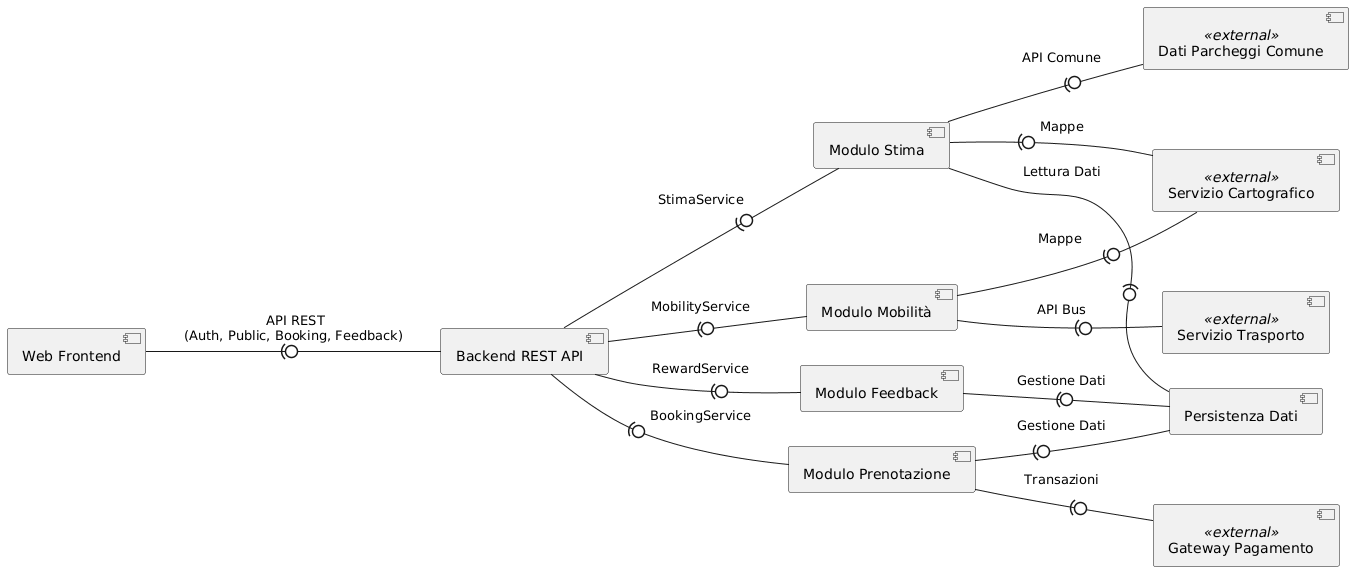
\includegraphics[width=\textwidth]{component_diagram.png}
    \caption{Diagramma dei componenti di TrentoParking}
    \label{fig:component-diagram}
\end{figure}

\subsection{Descrizione dei componenti}

\subsubsection{Web Frontend}
Il componente Web Frontend rappresenta il punto di accesso principale dell’utente. Permette di visualizzare la mappa, selezionare area e raggio, consultare la stima della disponibilità, ricevere suggerimenti di mobilità alternativa e, per gli utenti autenticati, inviare feedback o prenotare posti privati.

\paragraph{Interfacce fornite}
\begin{itemize}
    \item \textbf{UI}: interfaccia grafica accessibile da browser desktop e mobile.
\end{itemize}

\paragraph{Interfacce richieste}
\begin{itemize}
    \item \textbf{API REST}: interfaccia di accesso al backend, che comprende funzionalità di autenticazione, consultazione pubblica, prenotazione e feedback.
\end{itemize}

\subsubsection{Backend REST API}
Il Backend REST API espone le funzionalità del sistema tramite endpoint REST. Riceve le richieste dal frontend, valida i parametri in ingresso, coordina i moduli interni e restituisce le risposte in formato JSON. In questa vista architetturale, anche le operazioni amministrative sono veicolate attraverso il backend e non vengono rappresentate come interfaccia separata.

\paragraph{Interfacce fornite}
\begin{itemize}
    \item \textbf{API REST}: insieme delle operazioni di autenticazione, consultazione pubblica, gestione feedback e prenotazione.
\end{itemize}

\paragraph{Interfacce richieste}
\begin{itemize}
    \item \textbf{StimaService}
    \item \textbf{MobilityService}
    \item \textbf{RewardService}
    \item \textbf{BookingService}
\end{itemize}

\subsubsection{Modulo Stima}
Il Modulo Stima si occupa di elaborare la probabilità di trovare parcheggio gratuito o a pagamento in una determinata area. La stima viene ottenuta combinando dati esterni sui parcheggi, supporto cartografico e dati persistiti utili alla valutazione.

\paragraph{Interfacce fornite}
\begin{itemize}
    \item \textbf{StimaService}: servizio per la generazione della stima di disponibilità.
\end{itemize}

\paragraph{Interfacce richieste}
\begin{itemize}
    \item \textbf{API Comune}: accesso ai dati pubblici sui parcheggi del Comune.
    \item \textbf{Mappe}: supporto cartografico per geolocalizzazione e distanze.
    \item \textbf{Lettura Dati}: accesso ai dati persistiti necessari alla stima.
\end{itemize}

\subsubsection{Modulo Mobilità}
Il Modulo Mobilità viene attivato quando la disponibilità di parcheggio risulta bassa. Il suo compito è proporre un’alternativa basata sul trasporto pubblico, suggerendo linee e fermate utili a raggiungere la destinazione.

\paragraph{Interfacce fornite}
\begin{itemize}
    \item \textbf{MobilityService}: servizio per la generazione di suggerimenti di mobilità alternativa.
\end{itemize}

\paragraph{Interfacce richieste}
\begin{itemize}
    \item \textbf{Mappe}: supporto cartografico.
    \item \textbf{API Bus}: accesso ai dati del trasporto pubblico.
\end{itemize}

\subsubsection{Modulo Feedback}
Il Modulo Feedback gestisce l’inserimento, la modifica e la rimozione dei feedback da parte degli utenti autenticati, oltre all’aggiornamento del sistema di premialità.

\paragraph{Interfacce fornite}
\begin{itemize}
    \item \textbf{RewardService}: servizio di gestione feedback e premialità.
\end{itemize}

\paragraph{Interfacce richieste}
\begin{itemize}
    \item \textbf{Gestione Dati}: accesso ai dati persistiti relativi a utenti e feedback.
\end{itemize}

\subsubsection{Modulo Prenotazione}
Il Modulo Prenotazione rappresenta l’estensione demo innovativa del sistema. Quando la disponibilità di parcheggio è bassa, l’utente autenticato può visualizzare posti privati offerti da host e prenotarli. Il pagamento viene trattato come interazione con un servizio esterno mock.

\paragraph{Interfacce fornite}
\begin{itemize}
    \item \textbf{BookingService}: servizio per la gestione della prenotazione di posti privati.
\end{itemize}

\paragraph{Interfacce richieste}
\begin{itemize}
    \item \textbf{Gestione Dati}: accesso a utenti, posti privati e prenotazioni.
    \item \textbf{Transazioni}: interfaccia verso il gateway di pagamento mock.
\end{itemize}

\subsubsection{Persistenza Dati}
Il componente Persistenza Dati gestisce l’archiviazione delle informazioni applicative. Contiene dati relativi a utenti, feedback, parcheggi, posti privati, disponibilità orarie e prenotazioni.

\paragraph{Interfacce fornite}
\begin{itemize}
    \item \textbf{Lettura Dati}: interfaccia di accesso in lettura.
    \item \textbf{Gestione Dati}: interfaccia di accesso in lettura e scrittura.
\end{itemize}

\paragraph{Interfacce richieste}
\begin{itemize}
    \item Nessuna.
\end{itemize}

\subsubsection{Dati Parcheggi Comune}
Rappresenta il sistema esterno da cui vengono recuperati i dati sui parcheggi pubblici.

\paragraph{Interfacce fornite}
\begin{itemize}
    \item \textbf{API Comune}: accesso ai dati parcheggi.
\end{itemize}

\paragraph{Interfacce richieste}
\begin{itemize}
    \item Nessuna.
\end{itemize}

\subsubsection{Servizio Cartografico}
Rappresenta il sistema esterno usato per la visualizzazione geografica e il calcolo delle distanze.

\paragraph{Interfacce fornite}
\begin{itemize}
    \item \textbf{Mappe}: interfaccia cartografica.
\end{itemize}

\paragraph{Interfacce richieste}
\begin{itemize}
    \item Nessuna.
\end{itemize}

\subsubsection{Servizio Trasporto}
Rappresenta il sistema esterno che fornisce i dati sul trasporto pubblico.

\paragraph{Interfacce fornite}
\begin{itemize}
    \item \textbf{API Bus}: accesso ai dati del trasporto pubblico.
\end{itemize}

\paragraph{Interfacce richieste}
\begin{itemize}
    \item Nessuna.
\end{itemize}

\subsubsection{Gateway Pagamento}
Rappresenta il sistema esterno di pagamento mock utilizzato nella demo della prenotazione privata.

\paragraph{Interfacce fornite}
\begin{itemize}
    \item \textbf{Transazioni}: interfaccia per la gestione del pagamento.
\end{itemize}

\paragraph{Interfacce richieste}
\begin{itemize}
    \item Nessuna.
\end{itemize}

\section{Diagramma delle classi e descrizione delle classi}

In questa sezione viene descritta la struttura statica di TrentoParking, attraverso il diagramma delle classi e la descrizione delle classi principali. Il modello comprende le classi necessarie per autenticazione e ruoli, ricerca e stima, prenotazione privata e mobilità alternativa.

\subsection{Diagramma delle classi}

La Figura~\ref{fig:class-diagram} riporta il diagramma delle classi del sistema.

\begin{figure}[H]
    \centering
    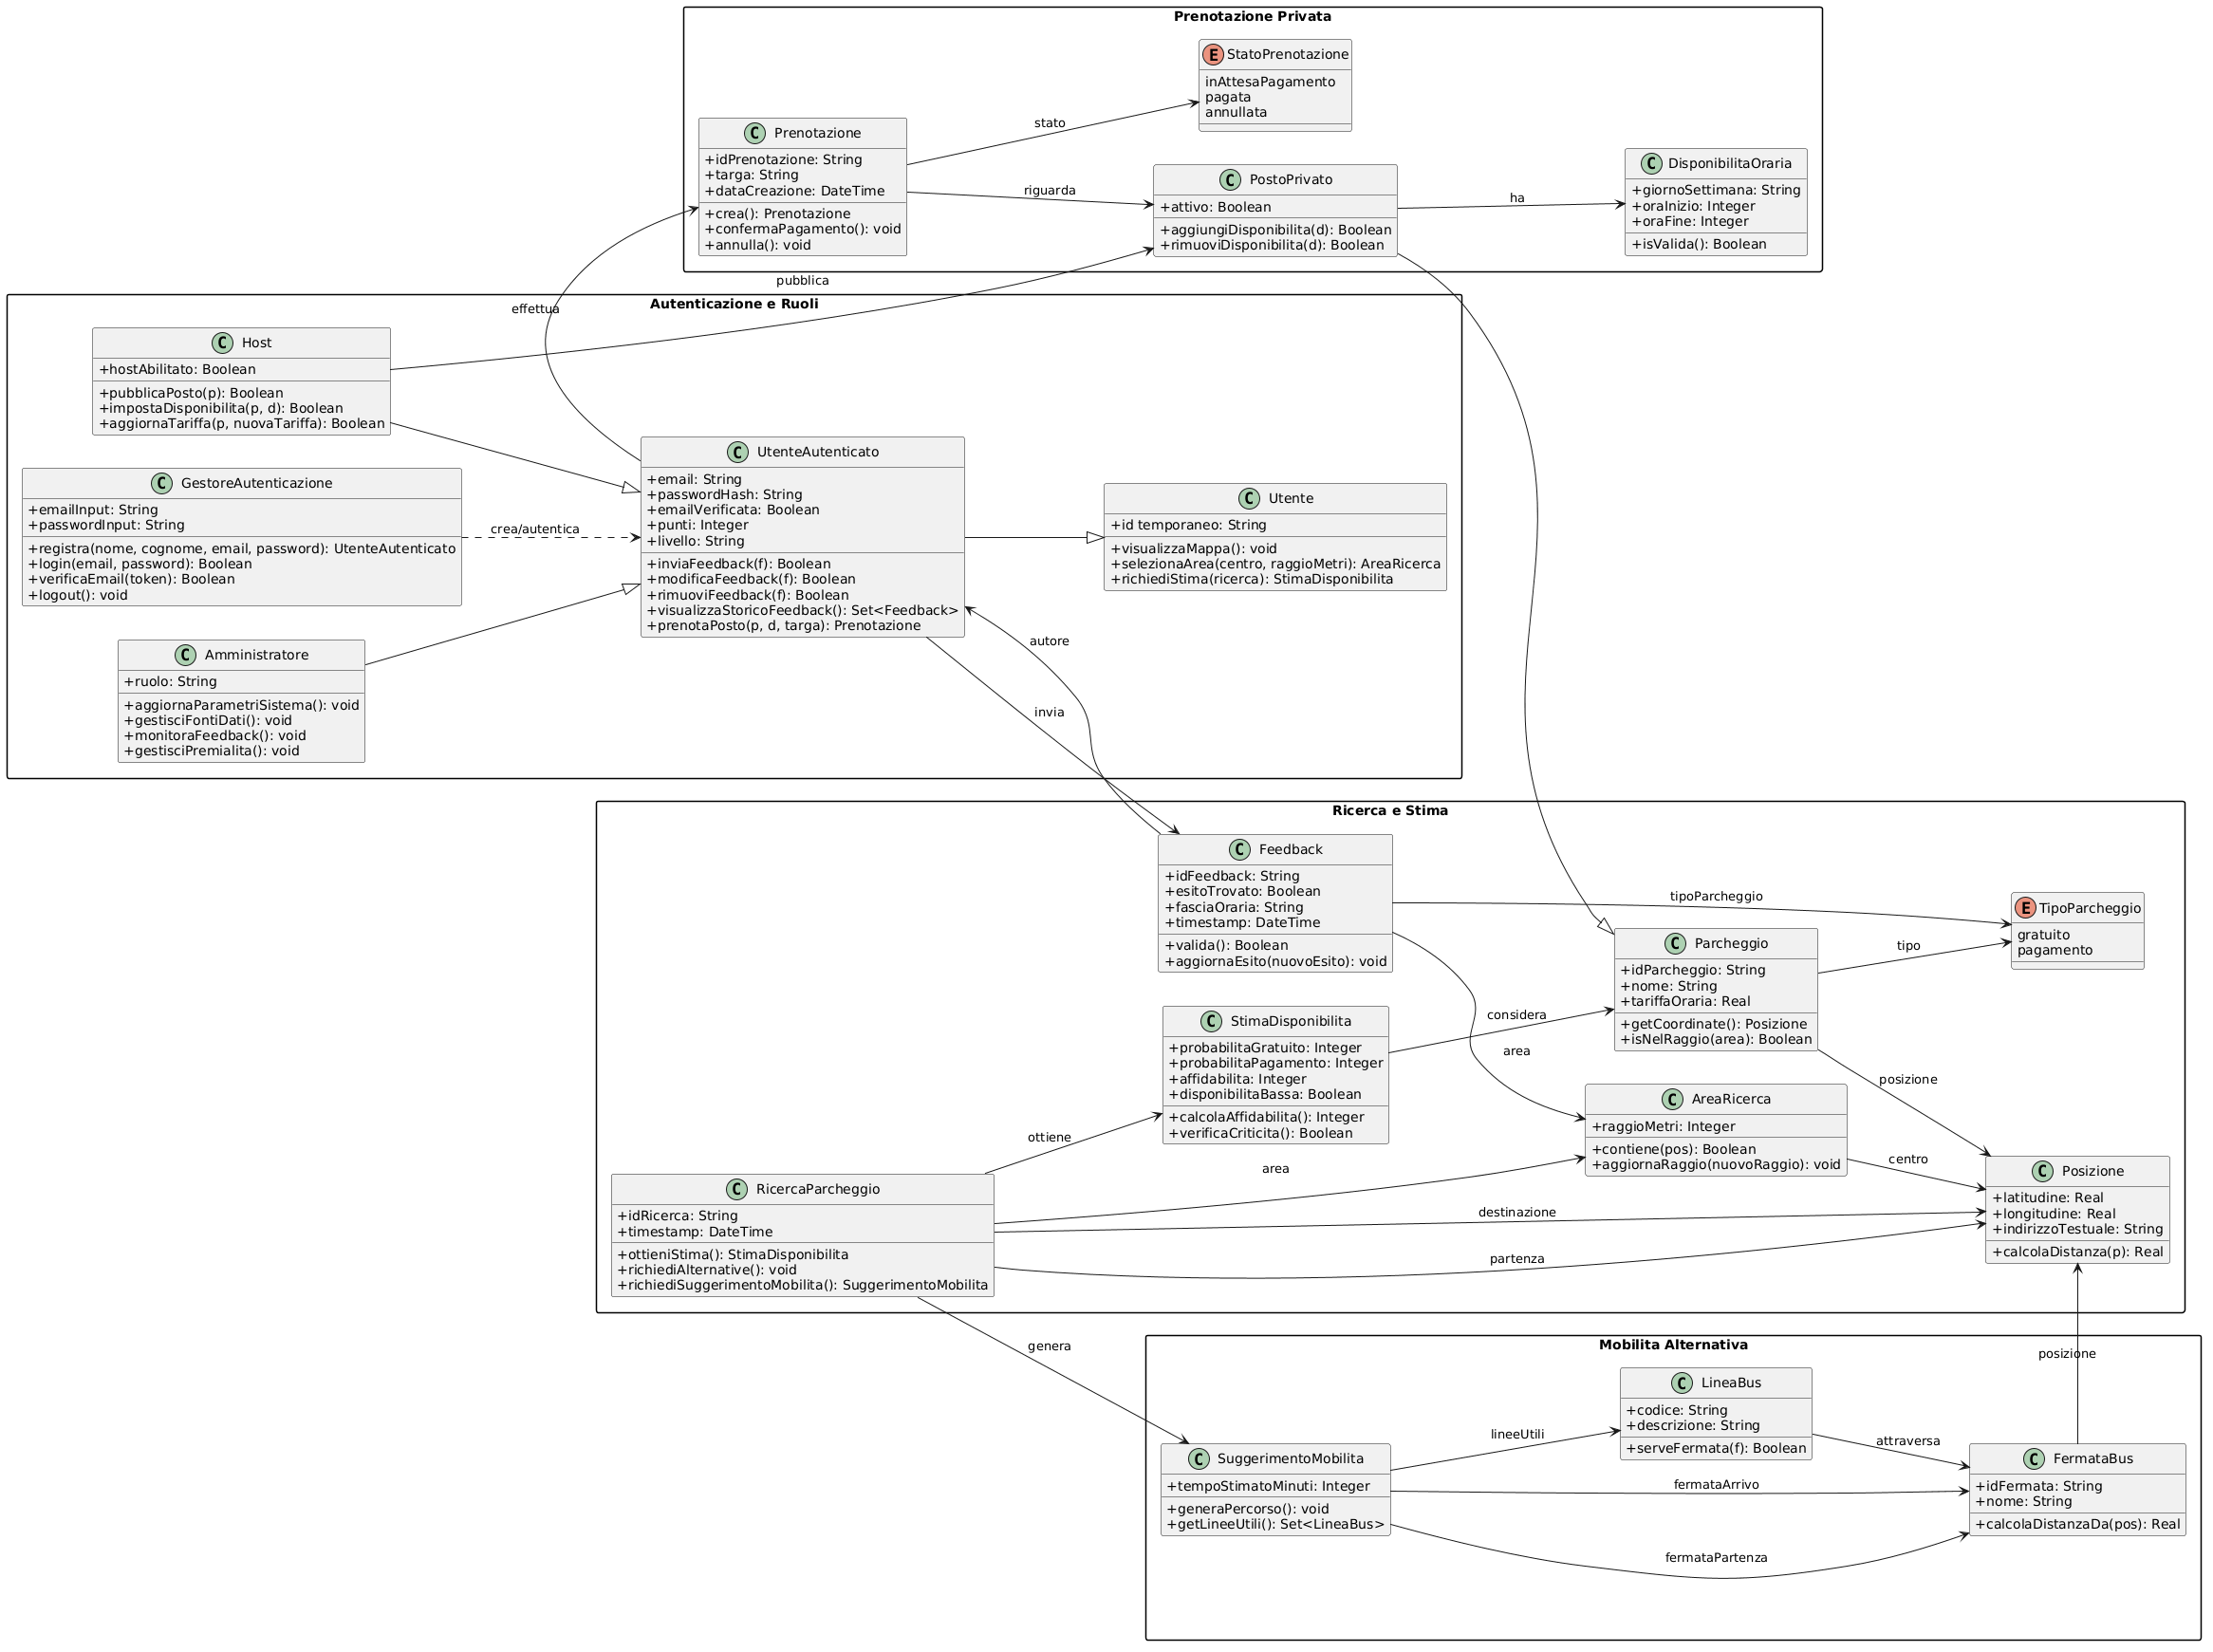
\includegraphics[width=\textwidth]{class_diagram.png}
    \caption{Diagramma delle classi di TrentoParking}
    \label{fig:class-diagram}
\end{figure}

\subsection{Autenticazione e Ruoli}

\subsubsection{GestoreAutenticazione}
Classe di controllo che gestisce registrazione, login, logout e verifica email.

\begin{itemize}
    \item \textbf{Attributi}: \texttt{emailInput: String}, \texttt{passwordInput: String}
    \item \textbf{Operazioni}:
    \begin{itemize}
        \item \texttt{registra(nome, cognome, email, password): UtenteAutenticato}
        \item \texttt{login(email, password): Boolean}
        \item \texttt{verificaEmail(token): Boolean}
        \item \texttt{logout(): void}
    \end{itemize}
\end{itemize}

\subsubsection{Utente}
Rappresenta l’utente generico del sistema, non necessariamente autenticato.

\begin{itemize}
    \item \textbf{Attributi}: \texttt{idTemporaneo: String}
    \item \textbf{Operazioni}:
    \begin{itemize}
        \item \texttt{visualizzaMappa(): void}
        \item \texttt{selezionaArea(centro, raggioMetri): AreaRicerca}
        \item \texttt{richiediStima(ricerca): StimaDisponibilita}
    \end{itemize}
\end{itemize}

\subsubsection{UtenteAutenticato}
Specializzazione di \texttt{Utente}. Accede alle funzionalità riservate del sistema.

\begin{itemize}
    \item \textbf{Attributi}: \texttt{email: String}, \texttt{passwordHash: String}, \texttt{emailVerificata: Boolean}, \texttt{punti: Integer}, \texttt{livello: String}
    \item \textbf{Operazioni}:
    \begin{itemize}
        \item \texttt{inviaFeedback(f): Boolean}
        \item \texttt{modificaFeedback(f): Boolean}
        \item \texttt{rimuoviFeedback(f): Boolean}
        \item \texttt{visualizzaStoricoFeedback(): Set<Feedback>}
        \item \texttt{prenotaPosto(p, d, targa): Prenotazione}
    \end{itemize}
\end{itemize}

\subsubsection{Host}
Specializzazione di \texttt{UtenteAutenticato}. Può offrire un proprio posto auto privato in determinate fasce orarie.

\begin{itemize}
    \item \textbf{Attributi}: \texttt{hostAbilitato: Boolean}
    \item \textbf{Operazioni}:
    \begin{itemize}
        \item \texttt{pubblicaPosto(p): Boolean}
        \item \texttt{impostaDisponibilita(p, d): Boolean}
        \item \texttt{aggiornaTariffa(p, nuovaTariffa): Boolean}
    \end{itemize}
\end{itemize}

\subsubsection{Amministratore}
Specializzazione di \texttt{UtenteAutenticato}. Gestisce parametri e fonti dati del sistema e controlla il meccanismo di premialità.

\begin{itemize}
    \item \textbf{Attributi}: \texttt{ruolo: String}
    \item \textbf{Operazioni}:
    \begin{itemize}
        \item \texttt{aggiornaParametriSistema(): void}
        \item \texttt{gestisciFontiDati(): void}
        \item \texttt{monitoraFeedback(): void}
        \item \texttt{gestisciPremialita(): void}
    \end{itemize}
\end{itemize}

\subsection{Prenotazione Privata}

\subsubsection{Prenotazione}
Rappresenta la prenotazione di un posto privato.

\begin{itemize}
    \item \textbf{Attributi}: \texttt{idPrenotazione: String}, \texttt{targa: String}, \texttt{dataCreazione: DateTime}
    \item \textbf{Operazioni}:
    \begin{itemize}
        \item \texttt{crea(): Prenotazione}
        \item \texttt{confermaPagamento(): void}
        \item \texttt{annulla(): void}
    \end{itemize}
\end{itemize}

La classe è associata a un posto privato e a uno stato di prenotazione.

\subsubsection{PostoPrivato}
Specializzazione di \texttt{Parcheggio}. Rappresenta un posto auto privato pubblicato da un host.

\begin{itemize}
    \item \textbf{Attributi}: \texttt{attivo: Boolean}
    \item \textbf{Operazioni}:
    \begin{itemize}
        \item \texttt{aggiungiDisponibilita(d): Boolean}
        \item \texttt{rimuoviDisponibilita(d): Boolean}
    \end{itemize}
\end{itemize}

La classe è associata a una o più disponibilità orarie.

\subsubsection{DisponibilitaOraria}
Rappresenta una fascia oraria in cui un posto privato è disponibile.

\begin{itemize}
    \item \textbf{Attributi}: \texttt{giornoSettimana: String}, \texttt{oraInizio: Integer}, \texttt{oraFine: Integer}
    \item \textbf{Operazioni}: \texttt{isValida(): Boolean}
\end{itemize}

\subsubsection{StatoPrenotazione}
Enumerazione che rappresenta lo stato di una prenotazione.

\begin{itemize}
    \item \textbf{Valori}: \texttt{inAttesaPagamento}, \texttt{pagata}, \texttt{annullata}
\end{itemize}

\subsection{Ricerca e Stima}

\subsubsection{RicercaParcheggio}
Rappresenta una richiesta di ricerca eseguita dall’utente.

\begin{itemize}
    \item \textbf{Attributi}: \texttt{idRicerca: String}, \texttt{timestamp: DateTime}
    \item \textbf{Operazioni}:
    \begin{itemize}
        \item \texttt{ottieniStima(): StimaDisponibilita}
        \item \texttt{richiediAlternative(): void}
        \item \texttt{richiediSuggerimentoMobilita(): SuggerimentoMobilita}
    \end{itemize}
\end{itemize}

La classe è associata a un’istanza di \texttt{AreaRicerca}, a una posizione di partenza, a una posizione di destinazione e può generare un suggerimento di mobilità.

\subsubsection{Feedback}
Rappresenta il contributo inviato da un utente autenticato sull’esito della ricerca di parcheggio.

\begin{itemize}
    \item \textbf{Attributi}: \texttt{idFeedback: String}, \texttt{esitoTrovato: Boolean}, \texttt{fasciaOraria: String}, \texttt{timestamp: DateTime}
    \item \textbf{Operazioni}:
    \begin{itemize}
        \item \texttt{valida(): Boolean}
        \item \texttt{aggiornaEsito(nuovoEsito): void}
    \end{itemize}
\end{itemize}

La classe è associata a un autore di tipo \texttt{UtenteAutenticato}, a un’area di ricerca e a una tipologia di parcheggio.

\subsubsection{StimaDisponibilita}
Contiene il risultato del calcolo effettuato dal sistema.

\begin{itemize}
    \item \textbf{Attributi}: \texttt{probabilitaGratuito: Integer}, \texttt{probabilitaPagamento: Integer}, \texttt{affidabilita: Integer}, \texttt{disponibilitaBassa: Boolean}
    \item \textbf{Operazioni}:
    \begin{itemize}
        \item \texttt{calcolaAffidabilita(): Integer}
        \item \texttt{verificaCriticita(): Boolean}
    \end{itemize}
\end{itemize}

La classe è associata ai parcheggi considerati per la stima.

\subsubsection{AreaRicerca}
Rappresenta l’area selezionata dall’utente.

\begin{itemize}
    \item \textbf{Attributi}: \texttt{raggioMetri: Integer}
    \item \textbf{Operazioni}:
    \begin{itemize}
        \item \texttt{contiene(pos): Boolean}
        \item \texttt{aggiornaRaggio(nuovoRaggio): void}
    \end{itemize}
\end{itemize}

La classe è associata a una posizione centrale.

\subsubsection{Parcheggio}
Rappresenta un parcheggio rilevante per la ricerca.

\begin{itemize}
    \item \textbf{Attributi}: \texttt{idParcheggio: String}, \texttt{nome: String}, \texttt{tariffaOraria: Real}
    \item \textbf{Operazioni}:
    \begin{itemize}
        \item \texttt{getCoordinate(): Posizione}
        \item \texttt{isNelRaggio(area): Boolean}
    \end{itemize}
\end{itemize}

La classe è associata a una posizione e a una tipologia di parcheggio.

\subsubsection{TipoParcheggio}
Enumerazione che distingue tra parcheggio gratuito e parcheggio a pagamento.

\begin{itemize}
    \item \textbf{Valori}: \texttt{gratuito}, \texttt{pagamento}
\end{itemize}

\subsubsection{Posizione}
Classe di supporto che rappresenta un punto geografico.

\begin{itemize}
    \item \textbf{Attributi}: \texttt{latitudine: Real}, \texttt{longitudine: Real}, \texttt{indirizzoTestuale: String}
    \item \textbf{Operazioni}: \texttt{calcolaDistanza(p): Real}
\end{itemize}

\subsection{Mobilità Alternativa}

\subsubsection{SuggerimentoMobilita}
Rappresenta l’alternativa di mobilità proposta dal sistema.

\begin{itemize}
    \item \textbf{Attributi}: \texttt{tempoStimatoMinuti: Integer}
    \item \textbf{Operazioni}:
    \begin{itemize}
        \item \texttt{generaPercorso(): void}
        \item \texttt{getLineeUtili(): Set<LineaBus>}
    \end{itemize}
\end{itemize}

La classe è associata a una fermata di partenza, una fermata di arrivo e a una o più linee bus utili.

\subsubsection{LineaBus}
Rappresenta una linea del trasporto pubblico.

\begin{itemize}
    \item \textbf{Attributi}: \texttt{codice: String}, \texttt{descrizione: String}
    \item \textbf{Operazioni}: \texttt{serveFermata(f): Boolean}
\end{itemize}

La classe è associata alle fermate attraversate.

\subsubsection{FermataBus}
Rappresenta una fermata del trasporto pubblico.

\begin{itemize}
    \item \textbf{Attributi}: \texttt{idFermata: String}, \texttt{nome: String}
    \item \textbf{Operazioni}: \texttt{calcolaDistanzaDa(pos): Real}
\end{itemize}

La classe è associata a una posizione geografica.

\section{Constraint OCL}

In questa sezione vengono riportati i vincoli OCL che completano il diagramma delle classi. I vincoli includono invarianti, precondizioni e postcondizioni.

\subsection{Area di ricerca valida}
Descrizione: il raggio di ricerca deve essere strettamente positivo.

\begin{verbatim}
context AreaRicerca
inv raggioPositivo: self.raggioMetri > 0
\end{verbatim}

\subsection{Coordinate geografiche valide}
Descrizione: le coordinate di una posizione devono rientrare negli intervalli geografici ammessi.

\begin{verbatim}
context Posizione
inv coordinateValide:
    self.latitudine >= -90 and self.latitudine <= 90 and
    self.longitudine >= -180 and self.longitudine <= 180
\end{verbatim}

\subsection{Tariffa coerente con il tipo di parcheggio}
Descrizione: se un parcheggio è gratuito, la tariffa oraria deve essere pari a zero.

\begin{verbatim}
context Parcheggio
inv tariffaCoerente:
    self.tipo = TipoParcheggio::gratuito implies self.tariffaOraria = 0
\end{verbatim}

\subsection{Probabilità di stima valide}
Descrizione: le probabilità stimate devono essere comprese tra 0 e 100.

\begin{verbatim}
context StimaDisponibilita
inv probabilitaValide:
    self.probabilitaGratuito >= 0 and self.probabilitaGratuito <= 100 and
    self.probabilitaPagamento >= 0 and self.probabilitaPagamento <= 100
\end{verbatim}

\subsection{Affidabilità valida}
Descrizione: anche il livello di affidabilità della stima deve essere compreso tra 0 e 100.

\begin{verbatim}
context StimaDisponibilita
inv affidabilitaValida:
    self.affidabilita >= 0 and self.affidabilita <= 100
\end{verbatim}

\subsection{Feedback completo}
Descrizione: ogni feedback deve essere associato a un’area e a una fascia oraria.

\begin{verbatim}
context Feedback
inv feedbackCompleto:
    self.area <> null and self.fasciaOraria <> ''
\end{verbatim}

\subsection{Invio feedback consentito solo a utenti verificati}
Descrizione: solo un utente autenticato con email verificata può inviare feedback.

\begin{verbatim}
context UtenteAutenticato::inviaFeedback(f: Feedback): Boolean
pre utenteVerificato:
    self.emailVerificata = true
\end{verbatim}

\subsection{Aggiornamento punti dopo il feedback}
Descrizione: un feedback valido incrementa il punteggio dell’utente.

\begin{verbatim}
context UtenteAutenticato::inviaFeedback(f: Feedback): Boolean
post puntiAggiornati:
    self.punti = self.punti@pre + 10
\end{verbatim}

\subsection{Punti non negativi}
Descrizione: il punteggio accumulato dall’utente deve essere sempre non negativo.

\begin{verbatim}
context UtenteAutenticato
inv puntiNonNegativi:
    self.punti >= 0
\end{verbatim}

\subsection{Fascia oraria valida}
Descrizione: una disponibilità oraria deve avere un’ora di inizio precedente all’ora di fine.

\begin{verbatim}
context DisponibilitaOraria
inv fasciaValida:
    self.oraInizio < self.oraFine
\end{verbatim}

\subsection{Prenotazione consentita solo a utenti verificati con targa inserita}
Descrizione: la prenotazione di un posto privato richiede email verificata e targa non vuota.

\begin{verbatim}
context UtenteAutenticato::prenotaPosto(p: PostoPrivato, d: DisponibilitaOraria, targa: String): Prenotazione
pre prenotazioneConsentita:
    self.emailVerificata = true and targa <> ''
\end{verbatim}

\subsection{Stato iniziale della prenotazione}
Descrizione: una nuova prenotazione viene creata nello stato iniziale di attesa pagamento.

\begin{verbatim}
context UtenteAutenticato::prenotaPosto(p: PostoPrivato, d: DisponibilitaOraria, targa: String): Prenotazione
post prenotazioneCreata:
    result.stato = StatoPrenotazione::inAttesaPagamento
\end{verbatim}

\end{document}